\documentclass{article} % set_input_method
\usepackage{hyperref}
\usepackage{graphicx}        % standard LaTeX graphics tool
\usepackage{enumitem}

\usepackage{xspace}
\newcommand{\ebkeyw}[1]{\textsf{\bfseries #1}}
\newcommand{\ebtag}[1]{\textcolor{pgrey}{\texttt{\bf #1}}}
\newcommand{\ebcode}[1]{\textsf{#1}}
\newcommand{\ebsets}[1]{\textsc{#1}}      % PERSON, BOOL
\newcommand{\ebcons}[1]{\textrm{#1}}      % john, TRUE, FALSE
\newcommand{\ebop}[1]{\textrm{\bfseries #1}}
\newcommand{\ebcmt}[1]{\textcolor{pgrey}{\textsf{\it #1}}}

\newcommand{\eb}{\textsf{Event-B}\xspace}
\newcommand{\jml}{\textsf{JML}\xspace}
\newcommand{\ebtj}{\textsf{Event\-B\-2\-Java}\xspace}
\newcommand{\javacode}[1]{\texttt{#1}}

\usepackage{amssymb}
\usepackage[utf8]{inputenc}
\newcommand{\continuation}{\rotatebox[origin=c]{90}{$\curvearrowleft$}}
\newcommand{\continuationR}{\rotatebox[origin=c]{-90}{$\curvearrowright$}}

\usepackage{color}
\definecolor{pgrey}{rgb}{0.75,0.75,0.75}

 \oddsidemargin 0pt % -10.4mm
 \evensidemargin 0pt % -10.4mm
 % \marginparwidth 0pts
 \marginparsep 0pt
 \topmargin 0mm % -10.4mm
 \headheight 0pt
 \headsep 0pt
 \textheight 232mm % 257.2mm
 \textwidth 165mm % 169.2mm
 \footskip 25pt %


\begin{document}

\begin{center}
\rule{\textwidth}{.0075in} \\
\rule[3mm]{\textwidth}{.0075in}\\

Universidade do Algarve\hfill Parallel and Distributed Systems \hfill 2026\\[3ex]

{\Large\bf Laboratório 1} \\[3ex]

\vspace*{0.30cm} Nome: 
  \raisebox{.2ex}{\makebox[0pt][l]{}}{\line(1,0){260}} \ %
  \textnumero:\line(1,0){50}

\rule{\textwidth}{.0075in} \\
\rule[3mm]{\textwidth}{.0075in} \\
\end{center}

\bigskip

\noindent
\textbf{Goal 1.} The first main goal of Recitation 1 (Laboratório 1) is for students to become familiar with the Rodin platform and the \eb language, including installing Rodin, configuring the necessary plugins, and understanding the basic environment and perspectives. Rodin is an IDE that provides supports for the modelling of systems and algorithms in \eb. We will be using \eb to model \textbf{distributed} algorithms and the Rodin platform to prove the correctness of these algorithms. 

\bigskip

\noindent
\textbf{Goal 2.} The second main goal of Recitation 1 (Laboratório 1) is for students to become familiar with the \ebtj code generator. This tool generates Java implementations for models written in \eb. Students will also learn how to use the generated code in the Eclipse IDE for Java.

\section{Installing Rodin on Windows}
\label{sec_rodin_windows}
%
Rodin is an Eclipse-based platform that supports the \eb formal language for writing \eb models, modelling safety invariants, and discharging proof obligations. We will be working with Rodin version 3.5 for editing and proving \eb models. Rodin is available for Windows, Linux, and Mac OS. You will be installing Rodin on your Windows machine. Alternatively, you can install Rodin on your Windows workspace as it is furnished by the UAlg. 

Rodin uses Java version 17, therefore, you will need to install Java version 17 before installing Rodin. You can install Java from  \href{https://adoptium.net/en-GB/temurin/releases?version=17} {https://\-adoptium.\-net/\-en-\-GB/\-temurin/\-releases?\-version=17}. Rodin 3.5 runs only on \texttt{x86\_64} machines, so make sure to select Java version 17 for \texttt{x86} machines and not for \verb+ARM64+ machines.

Download Rodin version 3.5 from \href{https://sourceforge.net/projects/rodin-b-sharp/files/Core_Rodin_Platform/3.5/} {https://\-source\-forge.\-net/\-pro\-jects/\-rodin\--b-\-sharp/\-files/\-Core\_\-Rodin\_\-Plat\-form/\-3.5/}. Next, you will need to tell Rodin to work with the Java version that you have just installed. Hence, edit Line 6 of the \verb+rodin.ini+ file as below.

\medskip
\noindent{
\begin{tabular}{l}
\verb+-Dosgi.requiredJavaVersion=17+
\end{tabular}}
\medskip


\section{Installing Rodin for Mac OS}
\label{sec_rodin_mac}

\index{Rodin}Rodin is an Eclipse-based platform that supports the \eb formal language for writing \eb models, modelling safety invariants, and discharging proof obligations with supported provers. This book works with Rodin version 3.5 for editing and proving \eb models and for generating code. Rodin 3.5 uses Java version 17, therefore, you will need to install Java version 17 before installing Rodin. Rodin 3.5 runs only on \texttt{x86\_64} Intel machines.

\medskip
\begin{tabular}{l}
\verb+curl -L -o OpenJDK17U-jdk_x64_mac_hotspot_17.0.17_10.pkg \+\\
\quad\quad\verb|https://github.com/adoptium/temurin17-binaries/|~~~\continuationR\\
\quad\quad\verb|releases/download/jdk-17.0.17+10/|~~~\continuationR\\
\verb|OpenJDK17U-jdk_x64_mac_hotspot_17.0.17_10.pkg|\\
\end{tabular}
\medskip

If your Mac is \verb+ARM64+, you will further need to install Rosetta to translate Intel \texttt{x86} instructions into \verb+ARM64+ instructions on Apple Silicon. We use a Mac mini M3 (Apple Silicon) as the reference platform, although the same procedure applies to other M1/M2/M3 systems. We install Rosetta as follows. 

\medskip
\verb+softwareupdate --install-rosetta --agree-to-license+
\medskip

Download Rodin version 3.5 for Mac from \href{https://sourceforge.net/projects/rodin-b-sharp/files/Core_Rodin_Platform/3.5/} {https://\-source\-forge.\-net/\-pro\-jects/\-rodin\--b-\-sharp/\-files/\-Core\_\-Rodin\_\-Plat\-form/\-3.5/}. Next, you need to set up Rodin to use Java 17. Thus, edit the file \texttt{rodin.\-app/\-Contents/\-Info.\-plist} as below.

\medskip
\begin{tabular}{l}
\verb+<string>+\\
  \verb+/Library/Java/JavaVirtualMachines/temurin-17.jdk/+~~~\continuationR\\
  \quad\quad\quad\verb+Contents/Home/bin/java+\\
\verb+</string>+\\
\end{tabular}
\medskip

Open the \verb+Rodin.app+. If you get a ``Rodin is damaged and can't be opened. You should move it to the Trash'' message, you can either go to \texttt{System Settings} $\rightarrow$ \texttt{Privacy \& Security} $\rightarrow$ \texttt{Security} $\rightarrow$ \texttt{Allow Anyway}, or you can type the following command line which removes the quarantine flag of the app. 

\medskip
\verb+sudo xattr -rd com.apple.quarantine rodin.app+
\medskip

%%%%%%%%%


\section{Installing Rodin on Linux}
\label{sec_rodin_linux}
Rodin 3.5 uses Java version 17, therefore, you will need to install Java version 17 before installing Rodin. Since you can have multiple versions of Java on your machine, we are going to install Java 17 separately.

Start by downloading the following tarball to any directory of your choice (\emph{e.g.} \texttt{$\sim$/Downloads}). \href{https://github.com/adoptium/temurin17-binaries/releases/download/jdk-17.0.18%2B8/OpenJDK17U-jdk_x64_linux_hotspot_17.0.18_8.tar.gz} {https://\-github.\-com/\-adoptium/\-temurin17-\-binaries/\-releases/\-download/\-jdk-\-17.\-0.18$\%$2B8/\-OpenJDK17U-\-jdk\_\-x64\_\-linux\_\-hotspot\_\-17.\-0.\-18\_8.\-tar\-.gz} 

\begin{itemize}
    %\item \texttt{wget https://github.com/adoptium/temurin17-binaries/releases/} ~\continuationR
    %\item[] \texttt{download/jdk-17.0.18\%2B8/OpenJDK17U-jdk\_x64\_linux\_hotspot\_17.0.1\_8.tar.gz}
    \item \texttt{sudo mkdir -p /opt/java}
    \item \texttt{sudo tar -xzf OpenJDK17U-jdk\_x64\_linux\_hotspot\_17.0.18\_8.tar.gz -C /opt/java}
\end{itemize}

Next, we are going to register both \texttt{java} and \texttt{javac} version 17 with \texttt{update-alternatives}. Moreover, we will use priority 1717 for an easier identification.

\begin{itemize}    
    \item \texttt{sudo update-alternatives --install /usr/bin/java java /opt/java/jdk-17.*/bin/java 1717}
    \item \texttt{sudo update-alternatives --install /usr/bin/javac javac /opt/java/jdk-17.*/bin/javac 1717}
\end{itemize}

Now, whenever we want to select Java 17, we perform the following commands:

\begin{itemize}    
    \item \texttt{sudo update-alternatives --config java}
    \begin{itemize}
        \item  choose the appropriate version (i.e. \texttt{/opt/java/jdk-17.../bin/java})
    \end{itemize}
    \item \texttt{sudo update-alternatives --config javac}
    \begin{itemize}
        \item  same thing for the compiler
    \end{itemize}
\end{itemize}

Finally, we will set \texttt{JAVA\_HOME} for Java 17 (after the following command do not forget to source the file).

\begin{verbatim}
    sudo tee /etc/profile.d/java17.sh <<'EOF'
    export JAVA_HOME=/opt/java/jdk-17
    export PATH=$JAVA_HOME/bin:$PATH
    EOF
\end{verbatim}

Download Rodin version 3.5 for Mac from \href{https://sourceforge.net/projects/rodin-b-sharp/files/Core_Rodin_Platform/3.5/rodin-3.5.0.202009111309-74e0e4188-linux.gtk.x86_64.tar.gz/download} {https://\-source\-forge.\-net/\-pro\-jects/\-rodin\--b-\-sharp/\-files/\-Core\_\-Rodin\_\-Plat\-form/\-3.5/}. Now, navigate to the destination folder and execute the following commands.

\begin{itemize}    
    \item \texttt{tar xvf rodin-3.5.0.202009111309-74e0e4188-linux.gtk.x86\_64.tar.gz}
    \item \texttt{sudo mv rodin /opt/rodin}
    \begin{itemize}
        \item let's make it system-wide and don't run it from \texttt{Downloads} like newbies.
    \end{itemize}
    \item \texttt{sudo ln -s /opt/rodin/rodin /usr/local/bin/rodin}
    \begin{itemize}
        \item this creates a symbolic link which allows us to start Rodin from anywhere just by typing \texttt{rodin}
    \end{itemize}
\end{itemize}



\section{Installing required plugins}
\label{subsec_plugins}

Rodin is an Eclipse IDE. Typical of Eclipse IDEs is the installation of additional functions via plugins. Before installing Rodin's required plugins, make sure you installed Java properly.

Open Rodin. Install the \emph{Camille} plugin via \texttt{Help} $\rightarrow$ \texttt{Install New Software} $\rightarrow$ \texttt{Add}, add the \href{https://www.stups.hhu.de/camille_updates} {https://\-www.\-stups.\-hhu.\-de/\-camille\_\-updates} Update Site, and follow the instructions. Camille is an editor for writing \eb models (as opposed to the structural editor that comes with Rodin). Restart Rodin after installing Camille.

Next, install the \emph{Atelier B Provers} plugin by using the \href{https://www.atelierb.eu/update_site/atelierb_provers} {https://\-www.\-atelierb.\-eu/\-update\_\-site/atelierb\_\-provers} Update Site and following the instructions as for Camille.

Last, install the Rodin's SMT solver using the Plug-Ins site \href{http://rodin-b-sharp.sourceforge.net/updates} {http://\-rodin-\-b-\-sharp.\-source\-forge.\-net/\-updates}. From the resulting menu select \texttt{Prover Extensions} $\rightarrow$ \texttt{SMT Solvers}. An SMT solver checks the satisfiability of logical formulas under theories like arithmetic, arrays or datatypes. 

\section{Installing EventB2Java}
\label{subsec_evenbt2java}
\ebtj is a code generator for \eb models. It is a Rodin plugin and only works with the version 3.5 of Rodin. To install \ebtj, you should download the \texttt{EventB\-2\-Java\-Jml\_\-plugin.\-jar} file that is available from the GitHub repository \href{https://github.com/ncatanoc/eventb2java}{https://\-github.\-com/\-ncatanoc/\-eventb\-2\-java} and drop it in the \texttt{dropins} directory of Rodin.

\begin{figure}
\centering 
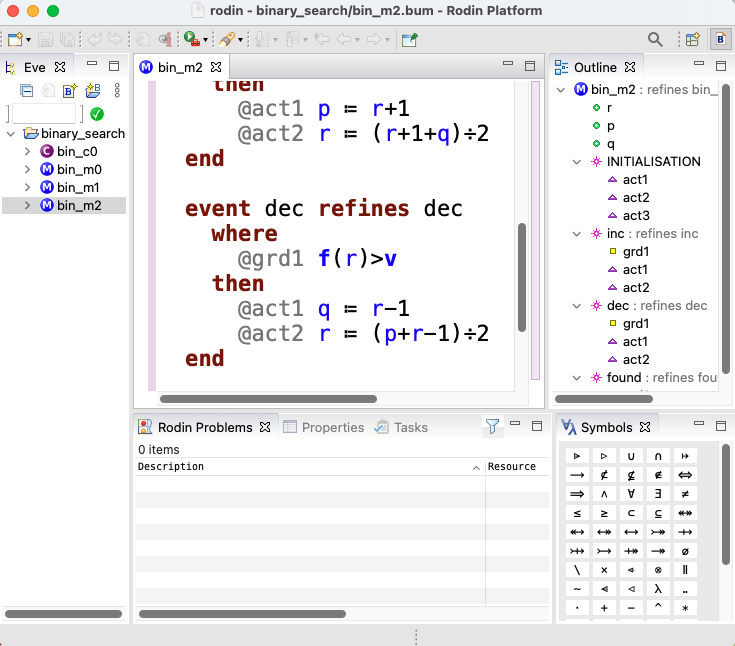
\includegraphics[width=10cm]{./figs/rodin_ide.png}
\caption{Rodin IDE}
\label{fig_rodin_ide}
\end{figure}

\section{Rodin's perspectives}
\label{subsec_rodin_perspectives}

Figure~\ref{fig_rodin_ide} shows the event \ebcode{dec} of the \emph{binary search} algorithm. The zip project of the binary search algorithm is available in the Tutoria system. Import it from Rodin: \texttt{File} $\rightarrow$ \texttt{Import} $\rightarrow$ \texttt{General} $\rightarrow$ \texttt{Existing Projects into Workspace} $\rightarrow$ \texttt{Browse} and select \texttt{binsearch.\-zip}. In Figure~\ref{fig_rodin_ide}, event \ebcode{dec} executes only when \ebtag{@grd1} \ebcode{f(r)} $>$  \ebcode{v}, where \ebcode{f} is an ordered array of elements, \ebcode{r} is an index in the array, and \ebcode{v} is the value the algorithm is searching for. The algorithm guarantees that \ebcode{r} is between \ebcode{p} and \ebcode{q}. Therefore, if \emph{guard} \ebtag{@grd1} holds, then the value \ebcode{v} is to the left of pivot \ebcode{r} and it is moved half way between \ebcode{p} and \ebcode{r}, and index \ebcode{q} is moved to the left of the previous value of \ebcode{r}.
The upper right part of Figure~\ref{fig_rodin_ide} shows that the current perspective is the \emph{Event-B} perspective (the blue B symbol in the upper right part). You can either manually switch to a particular perspective via \texttt{Window} $\rightarrow$ \texttt{Open Perspective} or undertake an action that causes the editor to automatically switch to a default perspective for that action. 

\begin{figure}[t]
  \centering
  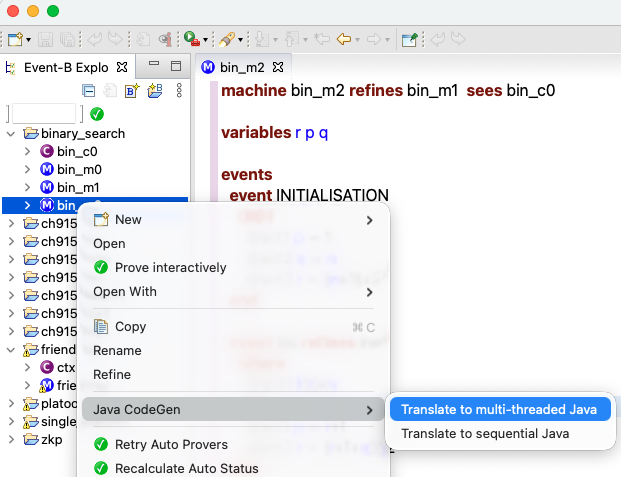
\includegraphics[width=10cm]{./figs/eventb2java_options.png}
  \caption{\ebtj: Java CodeGen}
  \label{fig_event2java_options}
\end{figure}

\section{Code generation with \ebtj}
\label{subsec_codegen}

Code generation with \ebtj works in the \emph{Event-B} perspective of Rodin, but the generated code is available in the \emph{Resource} perspective. To generate code for a specific \eb machine using \ebtj, in the Rodin Explorer panel of the \emph{Event-B} perspective, the user right-clicks the machine to generate code for it (see Figure~\ref{fig_event2java_options}), then selects \emph{Java CodeGen}, and finally chooses either \emph{Translate to multi-threaded Java} or \emph{Translate to sequential Java} from the context menu. \ebtj can generate code for machines at the different levels of abstraction, from the most abstract machine to the most concrete, for instance, the \texttt{Test\_\-bin\_\-m2.\-java} test class in Figure~\ref{fig_event2java_files}.

\ebtj translates each event as a Java \javacode{Thread} class implementation. Events can be triggered when their guards are satisfied, which results in the execution of the event actions. \ebtj models event triggering by creating two methods, a \javacode{guard} method containing the translation of the event guard, a \javacode{run} method containing the translation of the event body, e.g., \javacode{guard\_dec} and \javacode{run\_dec}.



\begin{figure}[t]
  \centering
  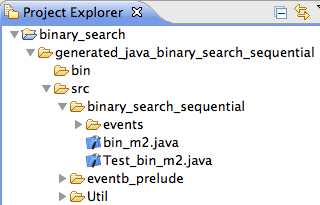
\includegraphics[width=8.5cm]{./figs/eventb2java_files.png}
  \caption{\ebtj: code structure}
  \label{fig_event2java_files}
\end{figure}

\section{Eclipse support}
\label{subsec_eclipse}

The whole code generated by \ebtj is an Eclipse project, which you can import from any Eclipse IDE for Java Developers \href{https://www.eclipse.org/downloads/packages/} {https://\-www.\-eclipse.\-org/\-downloads/\-packages/} via \texttt{File} $\rightarrow$ \texttt{Import} $\rightarrow$ \texttt{General} $\rightarrow$ \texttt{Existing Projects into Workspace}. The Eclipse project includes the \jml-specified Java code and the prelude libraries needed to execute the code. To access the code in Rodin, switch to the \emph{Resource} perspective via \texttt{Window} $\rightarrow$ \texttt{Perspective} $\rightarrow$ \texttt{Open Perspective}. The Eclipse project includes a folder named \texttt{generated\_\-java\_\-binary\_\-search} that contains the generated code, and an \texttt{eventb\_\-prelude} subfolder that contains the prelude Java implementation for \eb sets, relations, booleans, etc. (see Figure~\ref{fig_event2java_files}). The \texttt{events} package of the \texttt{src} subfolder contains the implementations of machine events. The file \texttt{bin\_\-m2.java} (\ebtj names this file after the corresponding machine in the \eb model) contains the Java code that creates the objects of the classes that represent the events and that declares machine variables and constants. \ebtj generates a test file \texttt{Test\_\-bin\_\-m2.java} that animates \texttt{bin\_\-m2.java}. 

\section*{Questions}
\label{subsec_questions}

\begin{enumerate}[label=(\alph*)]
\item \textbf{(1 point)} Install the Rodin IDE following Section~\ref{sec_rodin_windows} for Windows or Section~\ref{sec_rodin_mac} for Mac, and Section~\ref{subsec_plugins} in either case. Open Rodin and import the \eb model for the binary search algorithm: \texttt{File} $\rightarrow$ \texttt{Import} $\rightarrow$ \texttt{General} $\rightarrow$ \texttt{Existing Projects into Workspace} $\rightarrow$ \texttt{Browse} and select \texttt{binsearch.\-zip}. Rename your project (initially called \texttt{binary\_\-search} in the left-hand Rodin Explorer panel of the \emph{Event-B} perspective) to \texttt{student-\-number\_\-binary\_\-search}. For instance, \texttt{a85476\_\-binary\_\-search}, \texttt{a83892\_\-binary\_\-search}, etc. To rename your project, right-click on it and select \emph{Rename}. Take a snapshot of your Rodin IDE that shows $(i)$ the renamed binary search project, and $(ii)$ the content of the machine \texttt{bin\_\-m2} in the middle panel (double-click \texttt{bin\_\-m2}). Save the snapshot as \texttt{fig01.\-png} and place it in the folder \texttt{figs} in Overleaf.
  %
\begin{figure}[t]
  \centering
  
\includegraphics[width=16cm]{./figs/fig01.png}
  \caption{Answer to Question 1}
  \label{fig01}
\end{figure}
  %
\item \textbf{(1 point)} Rename the machine \texttt{bin\_\-m2} on the left-hand Rodin Explorer panel as \texttt{student-\-number\_\-bin\_\-m2}. For instance, name the machine \texttt{a66666\_\-bin\_\-m2} or \texttt{a62054\_\-bin\_\-m2}, etc. This renamed machine will be called \textbf{the second refinement machine}. Take a snapshot of your Rodin IDE in which the renamed machine is visible. Save the snapshot as \texttt{fig02.\-png} and place it in the folder \texttt{figs} in Overleaf.
%
\begin{figure}[ht]
  \centering
  
\includegraphics[width=16cm]{./figs/fig02.png}
  \caption{Answer to Question 2}
  \label{fig02}
\end{figure}


\item \textbf{(1 point)} Follow the instructions in Section~\ref{subsec_plugins} and install \ebtj. Follow the instructions in Section~\ref{subsec_codegen} to generate code for \textbf{the second refinement machine} created in the previous step. Therefore, in Rodin, right-click the second refinement machine and then select \texttt{Java CodeGen} $\rightarrow$ \texttt{Translate to multi-threaded Java} and wait for the ``Successful Translation'' pop-up window to be displayed. Then, switch to the \emph{Resource} perspective of Rodin: \texttt{Window} $\rightarrow$ \texttt{Perspective} $\rightarrow$ \texttt{Open Perspective} $\rightarrow$ \texttt{Resource}. Do not forget to \textbf{refresh} the \texttt{a66666\_\-binary\_\-search} project to visualise the generated code called \texttt{generated\_\-java\_\-a66666\_\-binary\_\-search\_\-multi\_\-threaded}!

Still in the \emph{Resource} perspective of Rodin, expand the folder \texttt{binary\_\-search\_\-multi\_\-threaded} and the \texttt{src} sub-folder therein to show all the Java classes. Take a snapshot of the \emph{Project Explorer} panel on the left-hand side of Rodin, and finally save the snapshot as \texttt{fig03.\-png} and place it in the folder \texttt{figs} in Overleaf.

\begin{figure}[ht]
  \centering
  
\includegraphics[width=16cm]{./figs/fig03.png}
  \caption{Answer to Question 3}
  \label{fig03}
\end{figure}

\item \textbf{(1 point)} Continuing from the previous point, you will generate an Eclipse project in the form of a zip file. Therefore, in the \emph{Project Explorer} panel of Rodin, right-click the project \texttt{generated\_\-java\_\-a66666\_\-binary\_\-search\_\-multi\_\-threaded} and select \texttt{Export} $\rightarrow$ \texttt{General} $\rightarrow$ \texttt{Archive File}, then save it as \texttt{generated\_\-java\_\-a66666\_\-binary\_\-search\_\-multi\_\-threaded.\-zip}. This zip file is an Eclipse project that will later be imported from Eclipse.

  Following Section~\ref{subsec_eclipse}, install an Eclipse IDE for Java on your laptop. In Eclipse, go to \texttt{File} $\rightarrow$ \texttt{Import} $\rightarrow$ \texttt{General} $\rightarrow$ \texttt{Existing Projects into Workspace} $\rightarrow$ \texttt{Select archive file} $\rightarrow$ \texttt{Browse}, then select your \texttt{generated\_\-java\_\-a66666\_\-binary\_\-search\_\-multi\_\-threaded.\-zip} file and import it.

Before moving on, in Eclipse, check your project in the \emph{Package Explorer} panel for any type of Java Build Path or Java Compiler error (search for any red cross). Right-click your \texttt{generated\_\-java\_\-a66666\_\-binary\_\-search\_\-multi\_\-threaded} Eclipse project and select \texttt{Properties} $\rightarrow$ \texttt{Java Compiler} to set an appropriate compiler compliance level, and ensure that a compatible JRE is selected. Make sure all red crosses disappear.

Within your \texttt{generated\_\-java\_\-a66666\_\-binary\_\-search\_\-multi\_\-threaded} Eclipse project, \textbf{expand} the Java classes in your \texttt{a66666\_\-binary\_\-search\_\-multi\_\-threaded} package. Take a snapshot of the \emph{Package Explorer} panel showing all the Java classes. Save the snapshot as \texttt{fig04.\-png} and place it in the folder \texttt{figs} in Overleaf. aaa bbb ccc.
  
\begin{figure}[ht]
  \centering
  
\includegraphics[width=16cm]{./figs/fig04.png}
  \caption{Answer to Question 4}
  \label{fig04}
\end{figure}

\item \textbf{(1 point)} In Eclipse, replace the method \verb+run_found+ in class \verb+found.java+ with the following code:

\begin{verbatim}
 public void run_found(){
  if(guard_found()) {
   System.out.println("found executed ");
   System.out.println("result = " +this.machine.get_r());
  }
  System.exit(1);
 }
\end{verbatim}

Edit the \texttt{Test*} class under the \texttt{a66666\_\-binary\_\-search\_\-multi\_\-threaded} package and replace the code of the method \texttt{main} with the following text.

\begin{verbatim}
/** User defined code that reflects axioms and theorems: Begin **/
test.random_f= new BRelation<Integer,Integer>();
test.random_f.add(new Pair<Integer, Integer>(0, 0)); 
test.random_f.add(new Pair<Integer, Integer>(1, 3));
test.random_f.add(new Pair<Integer, Integer>(2, 5));
test.random_f.add(new Pair<Integer, Integer>(3, 7));
test.random_f.add(new Pair<Integer, Integer>(4, 11));
test.random_f.add(new Pair<Integer, Integer>(5, 13));
test.random_f.add(new Pair<Integer, Integer>(6, 17));
test.random_v = 11;
test.random_n = 7;
/** User defined code that reflects axioms and theorems: End **/
\end{verbatim}

Run the \texttt{Test*} class under the \texttt{a66666\_\-binary\_\-search\_\-multi\_\-threaded} package: right-click \texttt{Test\_\-a66666\_\-bin\_\-m2.\-java}, then select \texttt{Run As} $\rightarrow$ \texttt{Java Application}. The result of the execution will be shown in the \emph{Console}. Take a snapshot of the \emph{Console}, save it as \texttt{fig05.\-png}, and place it in the folder \texttt{figs} in Overleaf.

\begin{figure}[ht]
  \centering
  
\includegraphics[width=16cm]{./figs/fig05.png}
  \caption{Answer to Question 5}
  \label{fig05}
\end{figure}

\end{enumerate}



\section*{What to turn in?}
\label{subsec_turnin}

\begin{enumerate}[label=(\alph*)]
\item Turn in a PDF created with Overleaf.
  %
\item Do not turn any source or additional file.  
\end{enumerate}  
  %


\end{document}
